\documentclass[12pt, conference]{IEEEtran}
\IEEEoverridecommandlockouts
% The preceding line is only needed to identify funding in the first footnote. If that is unneeded, please comment it out.
\usepackage{cite}
\usepackage{amsmath,amssymb,amsthm,amsfonts}
\usepackage{algorithm2e}
\usepackage{algorithm}
\usepackage{subfigure}
\usepackage{graphicx}
\usepackage{textcomp}
\usepackage{xcolor}
\usepackage{varwidth}
\usepackage{bookmark}
\usepackage[]{hyperref}
\hypersetup{
  bookmarks=true,
  bookmarksnumbered=true,     
  bookmarksopen=true,  
  colorlinks=false , 
  citecolor=.,   
  allbordercolors={white},               
  pdfstartview=Fit,           
  pdfpagemode=UseOutlines
}

  
  
\def\BibTeX{{\rm B\kern-.05em{\sc i\kern-.025em b}\kern-.08em
    T\kern-.1667em\lower.7ex\hbox{E}\kern-.125emX}}
\begin{document}

\title{WiFi Fingerprint Indoor Positioning System}

\author{\IEEEauthorblockN{Braxton Adams\textsuperscript{1}, Cyrus Cravens\textsuperscript{2}, Jonathan Adiri\textsuperscript{3}, Sang Xing\textsuperscript{4}}
  \IEEEauthorblockA{\textit{Department of Mathematics and Statistics}}
  {Portland State University, Portland, OR 97201 USA} \\
  \textsuperscript{1}braadams@pdx.edu, \textsuperscript{2}ccravens@pdx.edu, \textsuperscript{3}adiri@pdx.edu, \textsuperscript{4}sxing@pdx.edu
}

\maketitle



%------------------------------------------------------------------------------------------------------------------------------------
% Abstract and Keywords
%------------------------------------------------------------------------------------------------------------------------------------
\begin{abstract}
  To be continued...
\end{abstract}

\begin{IEEEkeywords}
  WiFi fingerprinting, WiFi indoor positioning, Trilateration, K-nearest neighbor algorithm
\end{IEEEkeywords}


%------------------------------------------------------------------------------------------------------------------------------------
% Introduction
%------------------------------------------------------------------------------------------------------------------------------------
\section{Introduction}
In recent years, with the ubiquity of mobile and Internet of Things devices, the possibility of creating an Indoor Positioning System (IPS), has become a reality for many structures. Our client, the engineering department of a university, has requested our team to create a model that predicts the physical location of a device, based on a set of signal strengths between access points and connected devices. The client also asked our team to quantify the accuracy and precision of the model. In order to find the most accurate way of predicting the location, two approaches were used in this experiment, Trilateration and the K-nearest Neighbors algorithm (KNN) and The experimental results showa that our model has been able to predict the location of a connected device to an average positioning error of 8 feet.

Our group was contacted by a local university who collected data from their internet network. The client requested that we identify the physical location of devices that are connected to the university network. There are six access points (i.e. wifi routers), with distinct MAC addresses, on a certain floor of one of the university buildings. The floor-plan is roughly 35mx18m and is composed of several class rooms and hallways. Devices that are connected to the network can measure the Received Signal Strength Indication (RSSI) of all access points within range. To collect the data, a mobile device connected to the network has recorded different values at various locations and oriented in various directions. The collected data was split into Offline and Online data, which will later be used to train and test the models developed by our team.
Two approaches were tried. The first, Trilateration, is the use of distances for determining the coordinates of a point in space. Since this approach is being used for geopositioning, we thought that it might be applied to IPS as well. The second approach, KNN, is a non-parametric supervised learning method. This approach seems promising because it has been proven successful in the past at solving similar problems.


%------------------------------------------------------------------------------------------------------------------------------------
% Data
%------------------------------------------------------------------------------------------------------------------------------------
\section{Data}

\begin{figure}[htbp]
  \centering
  \subfigure[00:0f:a3:39:e1:c0]{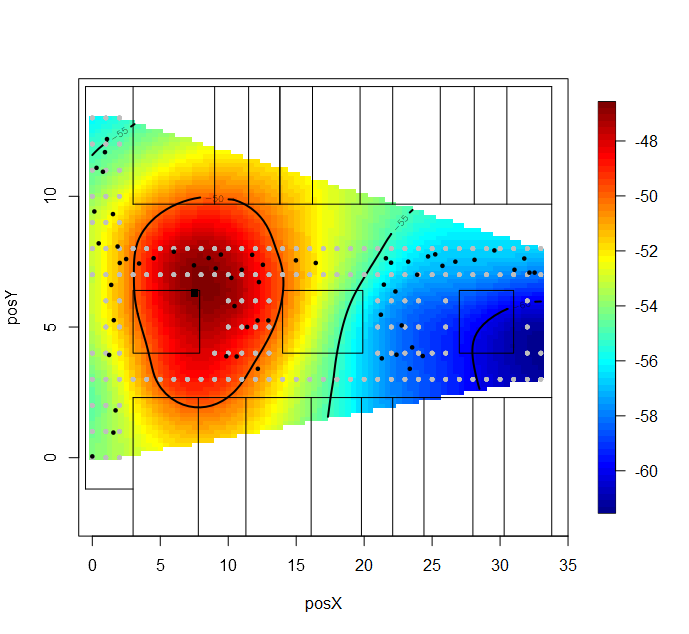
\includegraphics[width=0.24\textwidth]{img/heatMap_allMac_8Angles/Mac-1.png}}
  \subfigure[00:14:bf:b1:97:8a]{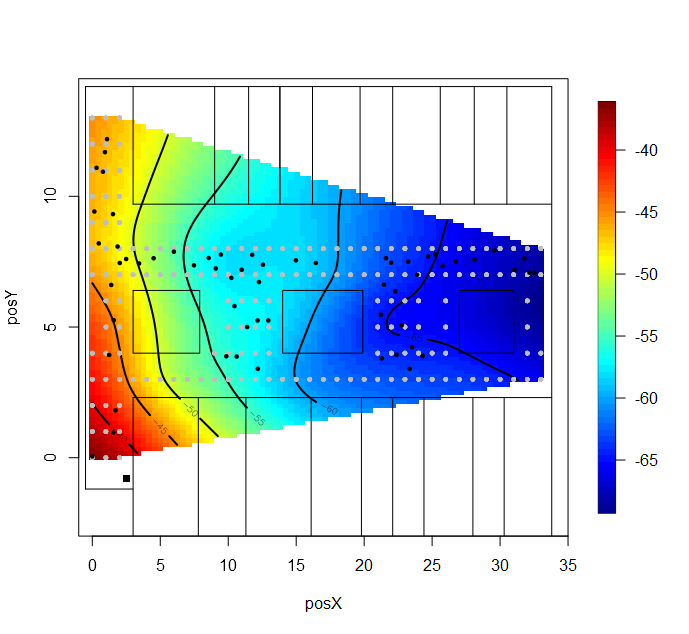
\includegraphics[width=0.24\textwidth]{img/heatMap_allMac_8Angles/Mac-2.png}}
  \subfigure[00:14:bf:3b:c7:c6]{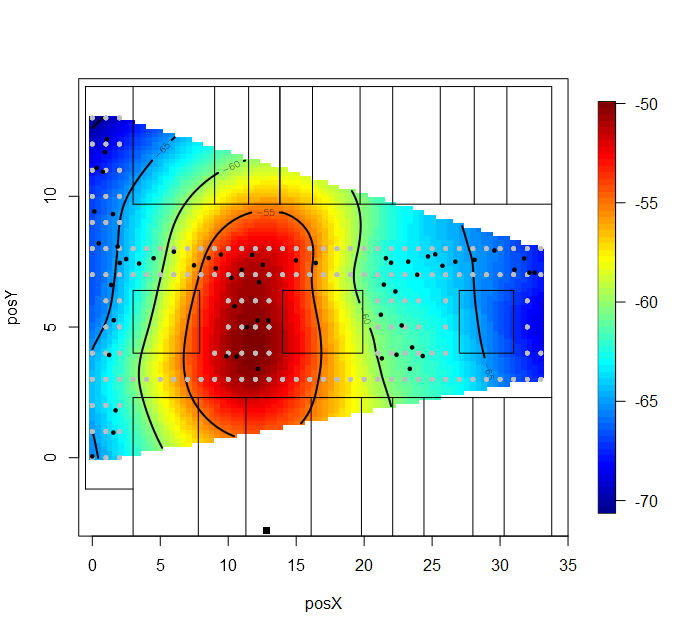
\includegraphics[width=0.24\textwidth]{img/heatMap_allMac_8Angles/Mac-3.png}}
  \subfigure[00:14:bf:b1:97:90]{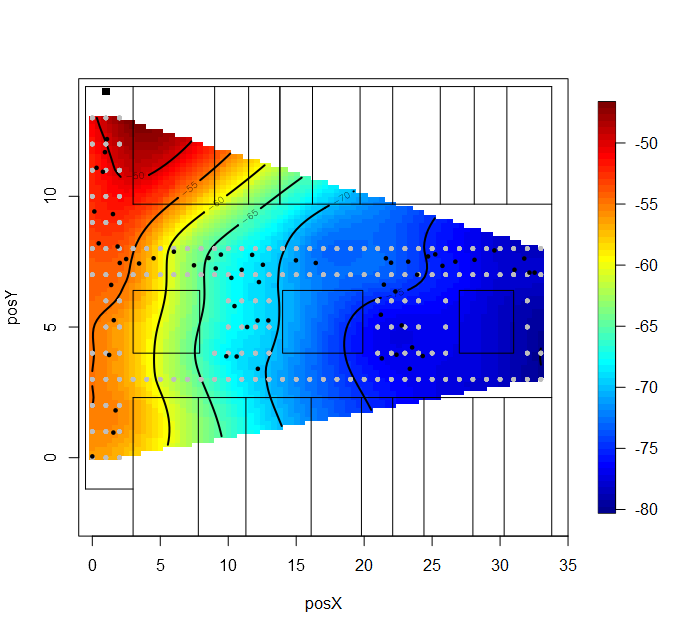
\includegraphics[width=0.24\textwidth]{img/heatMap_allMac_8Angles/Mac-4.png}}
  \subfigure[00:14:bf:b1:97:8d]{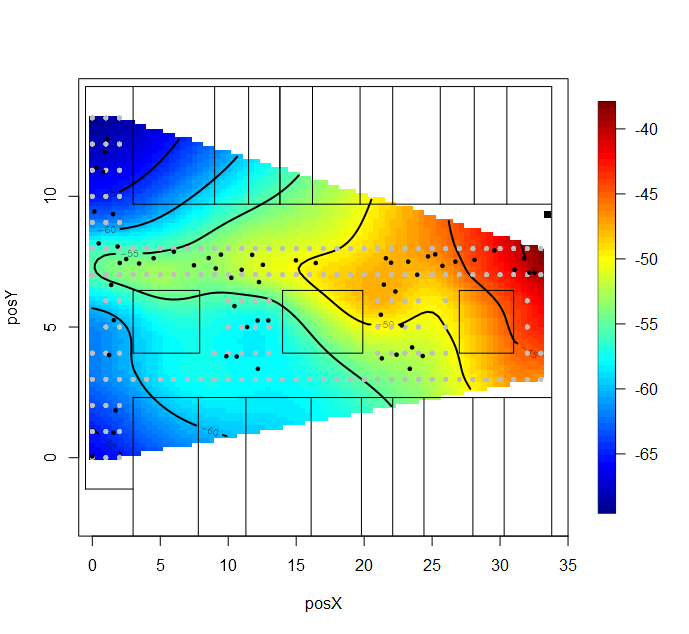
\includegraphics[width=0.24\textwidth]{img/heatMap_allMac_8Angles/Mac-5.png}}
  \subfigure[00:14:bf:b1:97:81]{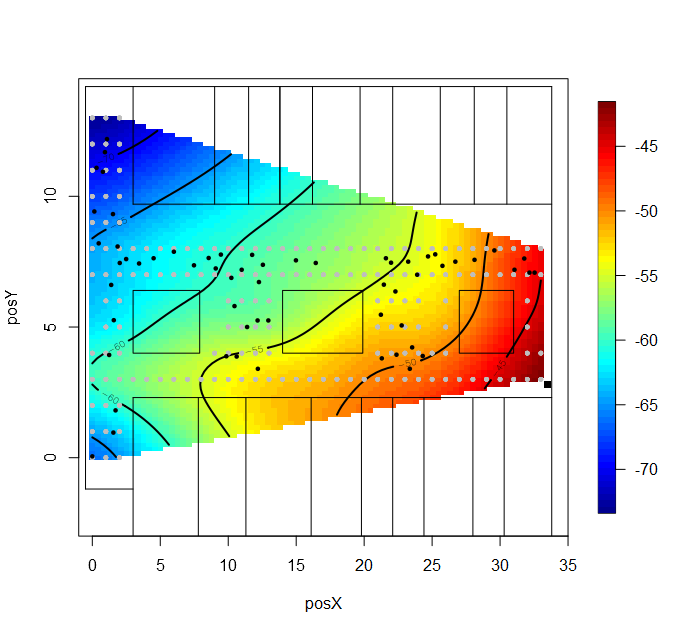
\includegraphics[width=0.24\textwidth]{img/heatMap_allMac_8Angles/Mac-6.png}}
  \caption{Heat map of 6 Access Points in all orientations}
  \label{fig: Heat Map of 6 APs}
\end{figure}


%------------------------------------------------------------------------------------------------------------------------------------
% Methodology
%------------------------------------------------------------------------------------------------------------------------------------
\section{Methodology}
\begin{itemize}
  \item Concise and intuitive description of methods considered
  \item Results
  \item Re-state the points of project and show how these were tackled and what resulted from analysis
  \item Include most relevant results to display, others go in appendix
\end{itemize}
\newline

There are many different statistical techniques we can use to estimate the location of a device from the detected RSSIs between the device and several access points. Another method we adopted is using the K-nearest Neighbors (KNN) Classification algorithm in order to predict the locations of our devices from the online dataset. The procedure of this method is as follows: we first have our entire dataset consisting of offline and online data, we these transform the offline data as our training dataset and online data as our testing dataset. Since the testing dataset has records of RSSI values from various locations, we take these RSSI values compare with the close neighbors (in terms of RSSI) from out training dataset. By close, we mean finding similar RSSI values from training dataset under the assumption that the predicted location has the same MAC address and orientation as the actual location of the testing dataset. We define $k$ as the number of neighbors in the training set, then the corresponding positions of our neighbors will be considered as the predicted positions in the test dataset. The neighbors are defines to be 
$$
  \text{min}\left(\sqrt{(RSSI_{train}-RSSI_{test})^2}\right), k=1.
$$ 
If $k>1$, then we choose least k numbers of RSSI values as our neighbors.


Now that we have the basic procedures as to how to find the predicted positions, this brings up a new question as to how many neighbors should we select? The choice of $k$ is very sensitive, choosing a small amount of $k$ leads to underfitting of our model to the training data, and choosing a large amount of $k$ leads to overfitting. Ideally, we want to choose the value of $k$ that is independent from our test data, the method of $k$-fold Cross-Validation (CV) can help us do this.

The idea behind $k$-fold CV is quite simple: we first divide our training data into numerous non-overlapping subsets of equal size. Then for each subset, we build models with the data that are not in that subset and we assess the predictive ability of the model using the subset that was left out. We repeat this model fitting and assessment for each folds and aggregate the prediction errors across the folds. The prediction errors are denoted as 
$$
  \text{SSE}(XY_{act}-XY_{est}),
$$ 
where SSE stands for Sum of Sqaures Error or Sum of Sqaures Residuals, representing the difference between the actual postilion and the estimated position of devices (see Fig~\ref{fig: K-Fold CV}).
\begin{figure}[htbp]
  \centerline{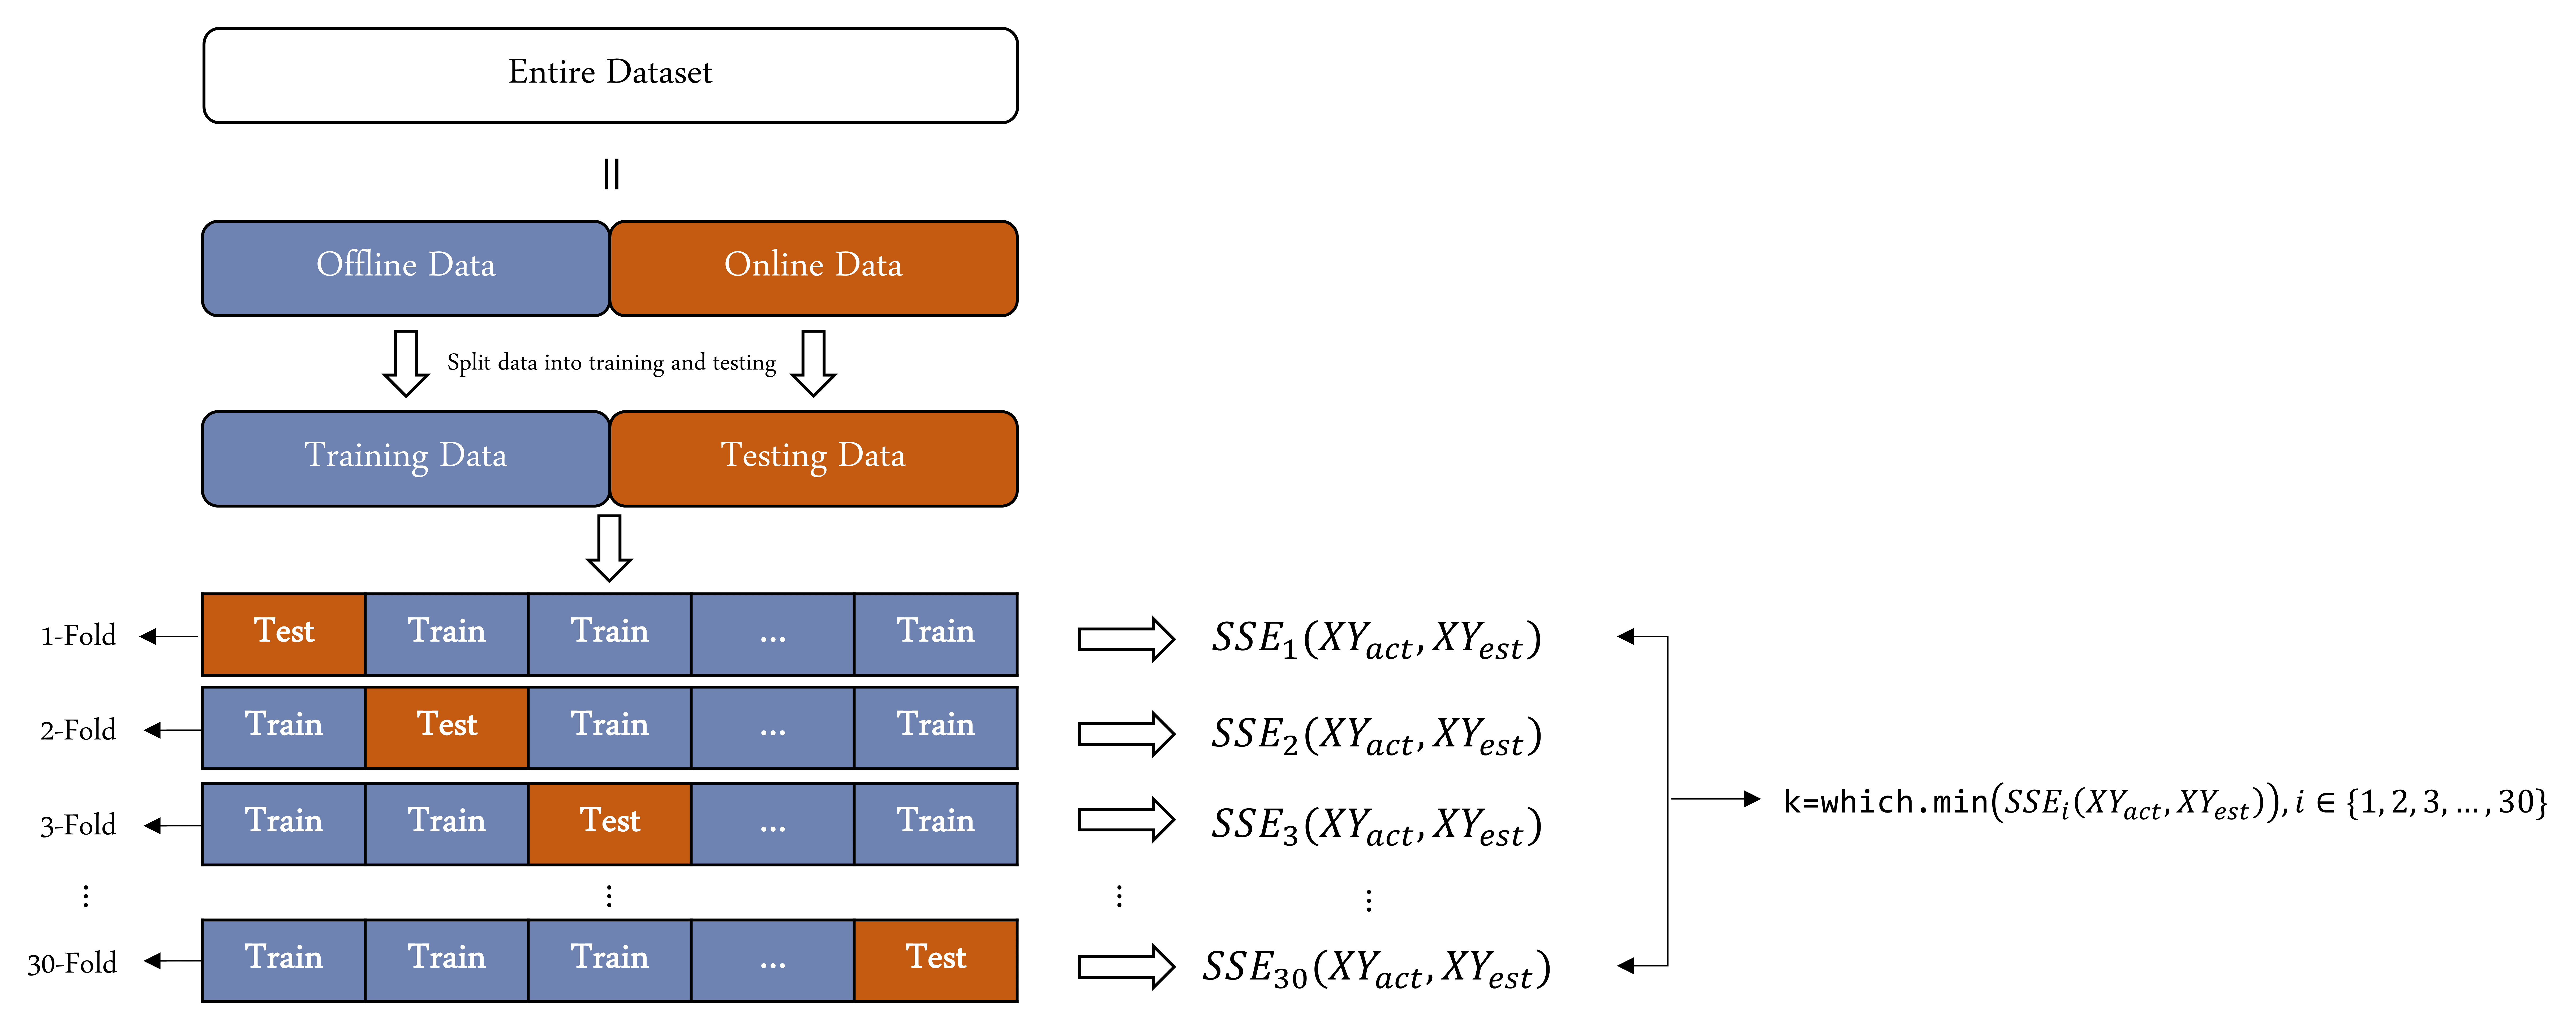
\includegraphics[width=\columnwidth]{img/K-Fold CV.png}}
  \caption{Schematic diagram of K-fold Cross-Validation}
  \label{fig: K-Fold CV}
\end{figure}

\begin{figure}[htbp]
  \centerline{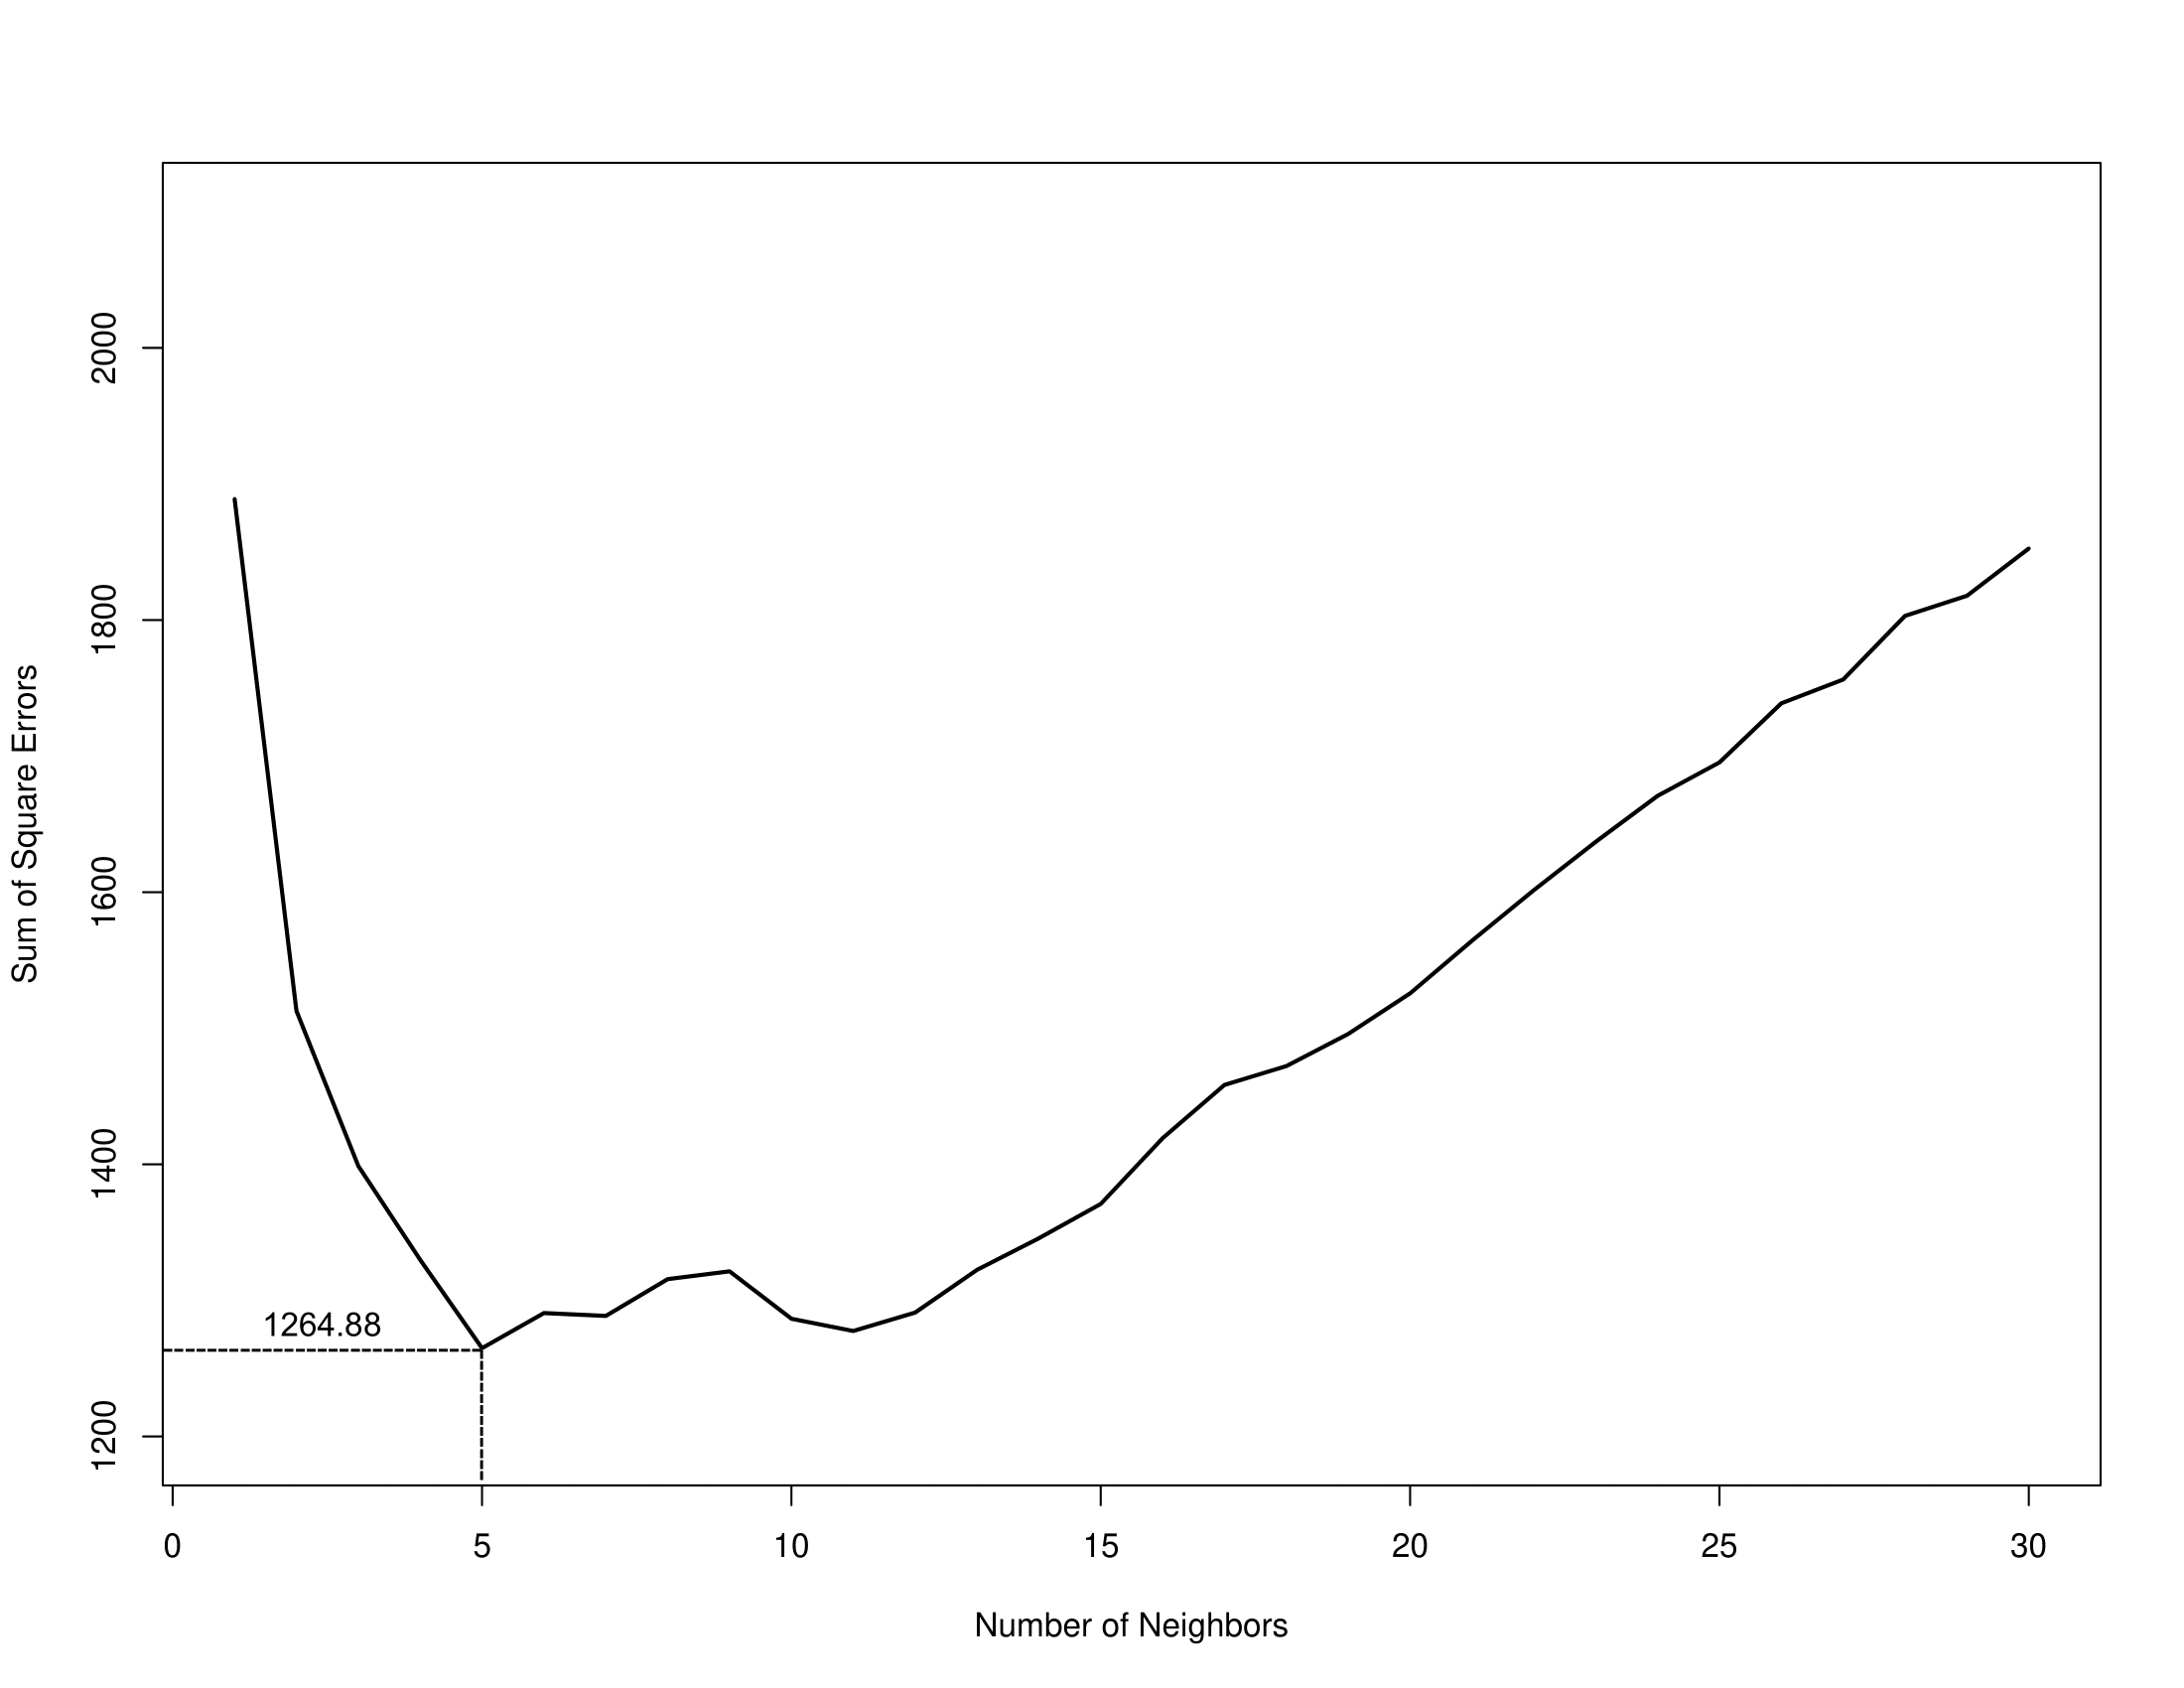
\includegraphics[width=\columnwidth]{img/Plot-k-fold_CV-1.png}}
  \caption{Schematic diagram of K-fold Cross-Validation}
  \label{fig: Choice of K}
\end{figure}
As the above figure shows, the SSE is lowest when $k=5$, hinting us that 5 neighbors will give us the least error between estimated positions and actual positions.

\begin{figure}[htbp]
  \centerline{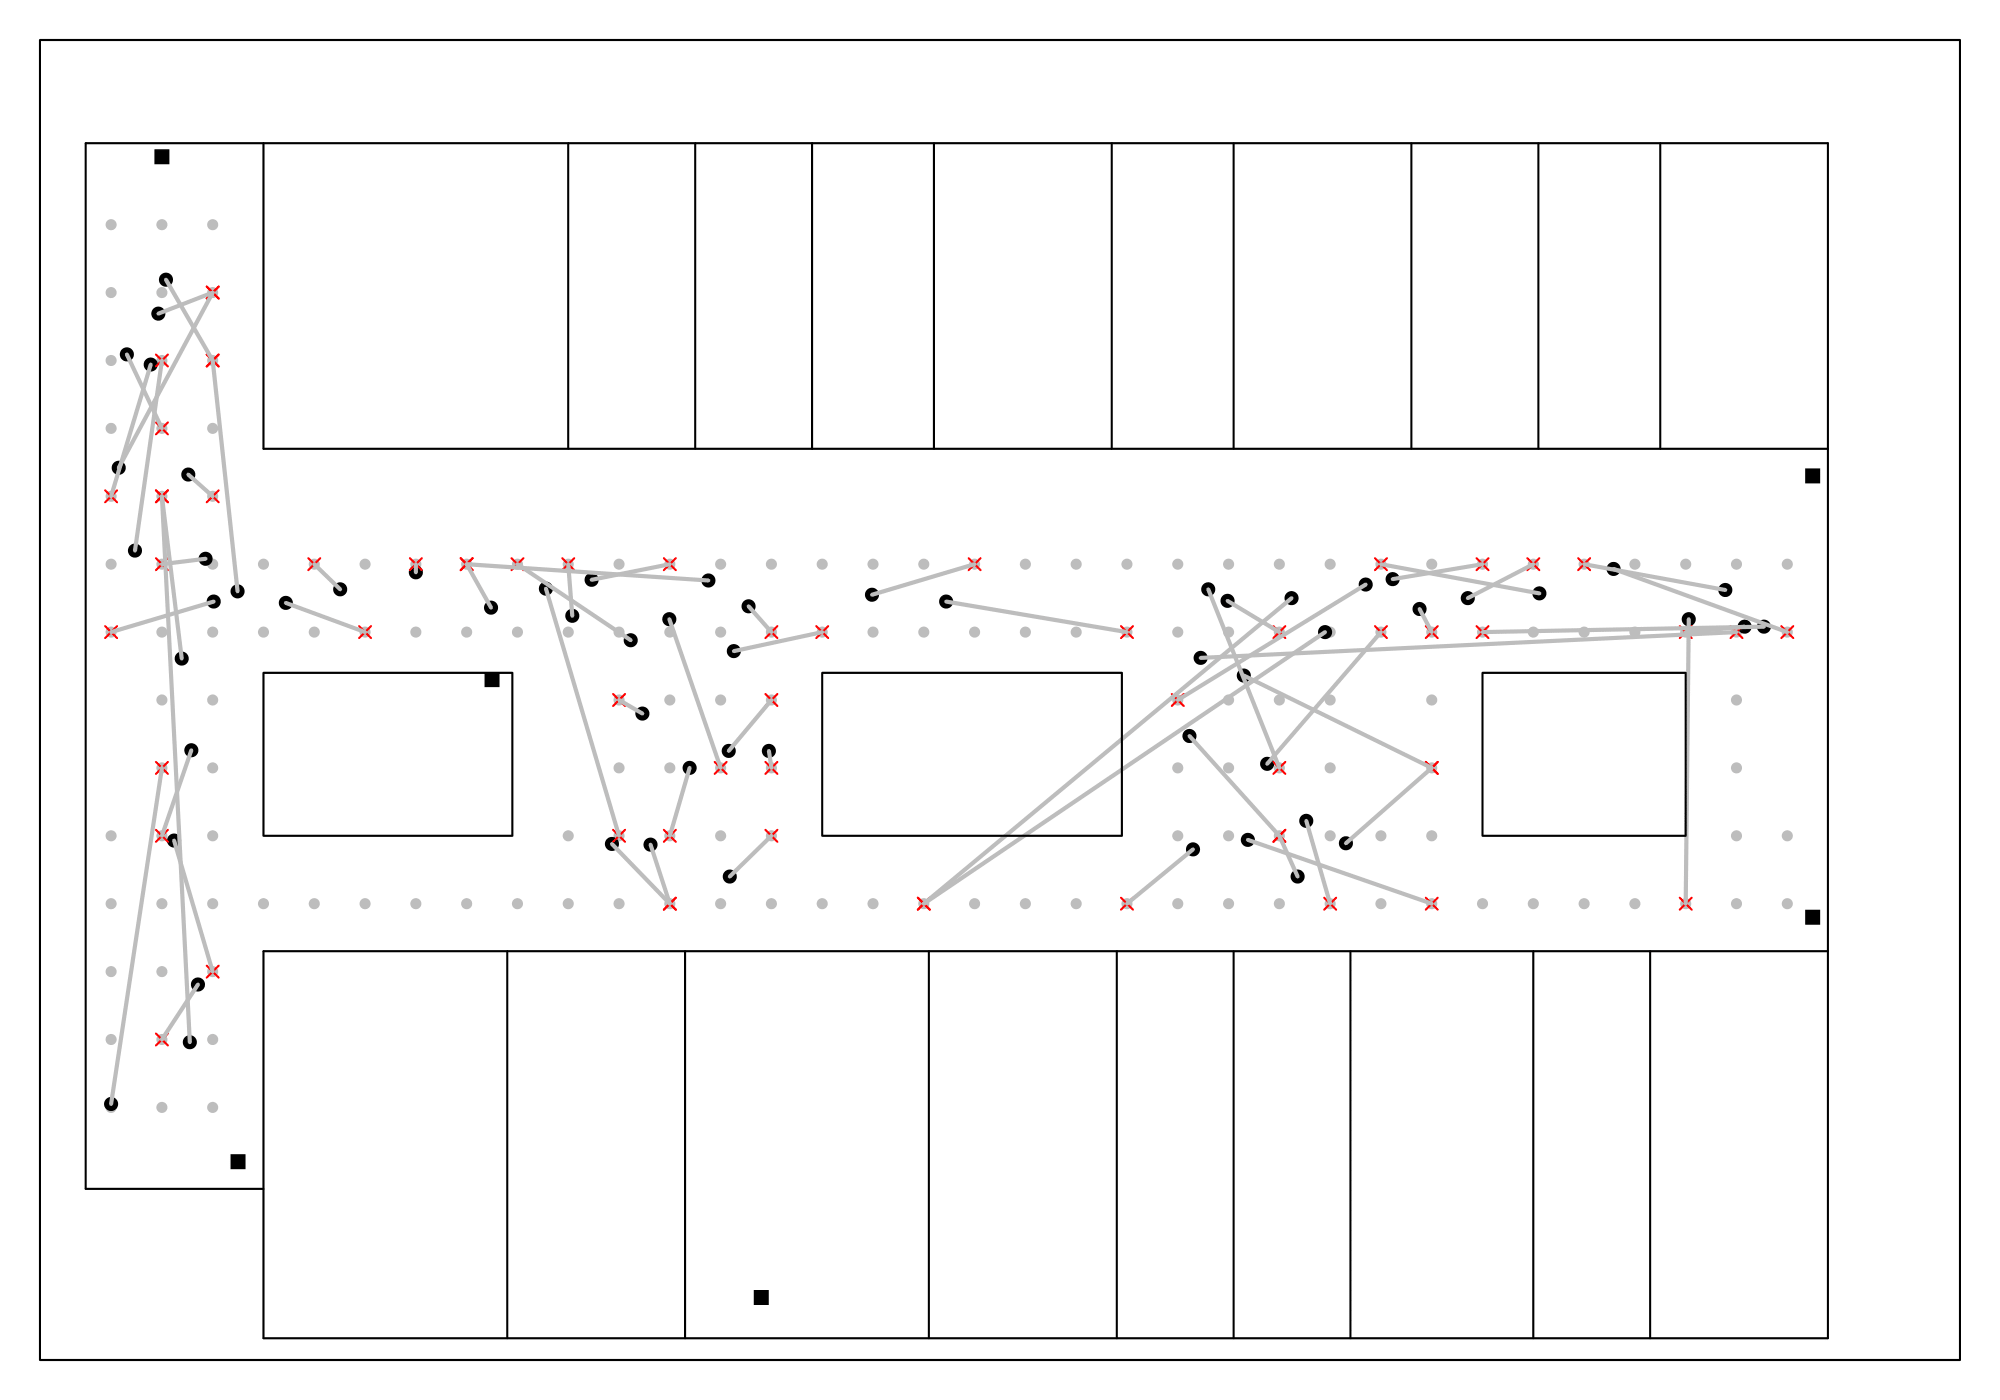
\includegraphics[width=\columnwidth]{img/Plot-K1FloorPlan-1.png}}
  \caption{Floor plan of estimated device locations when $k=1$}
  \label{fig: K1}
\end{figure}

\begin{figure}[htbp]
  \centerline{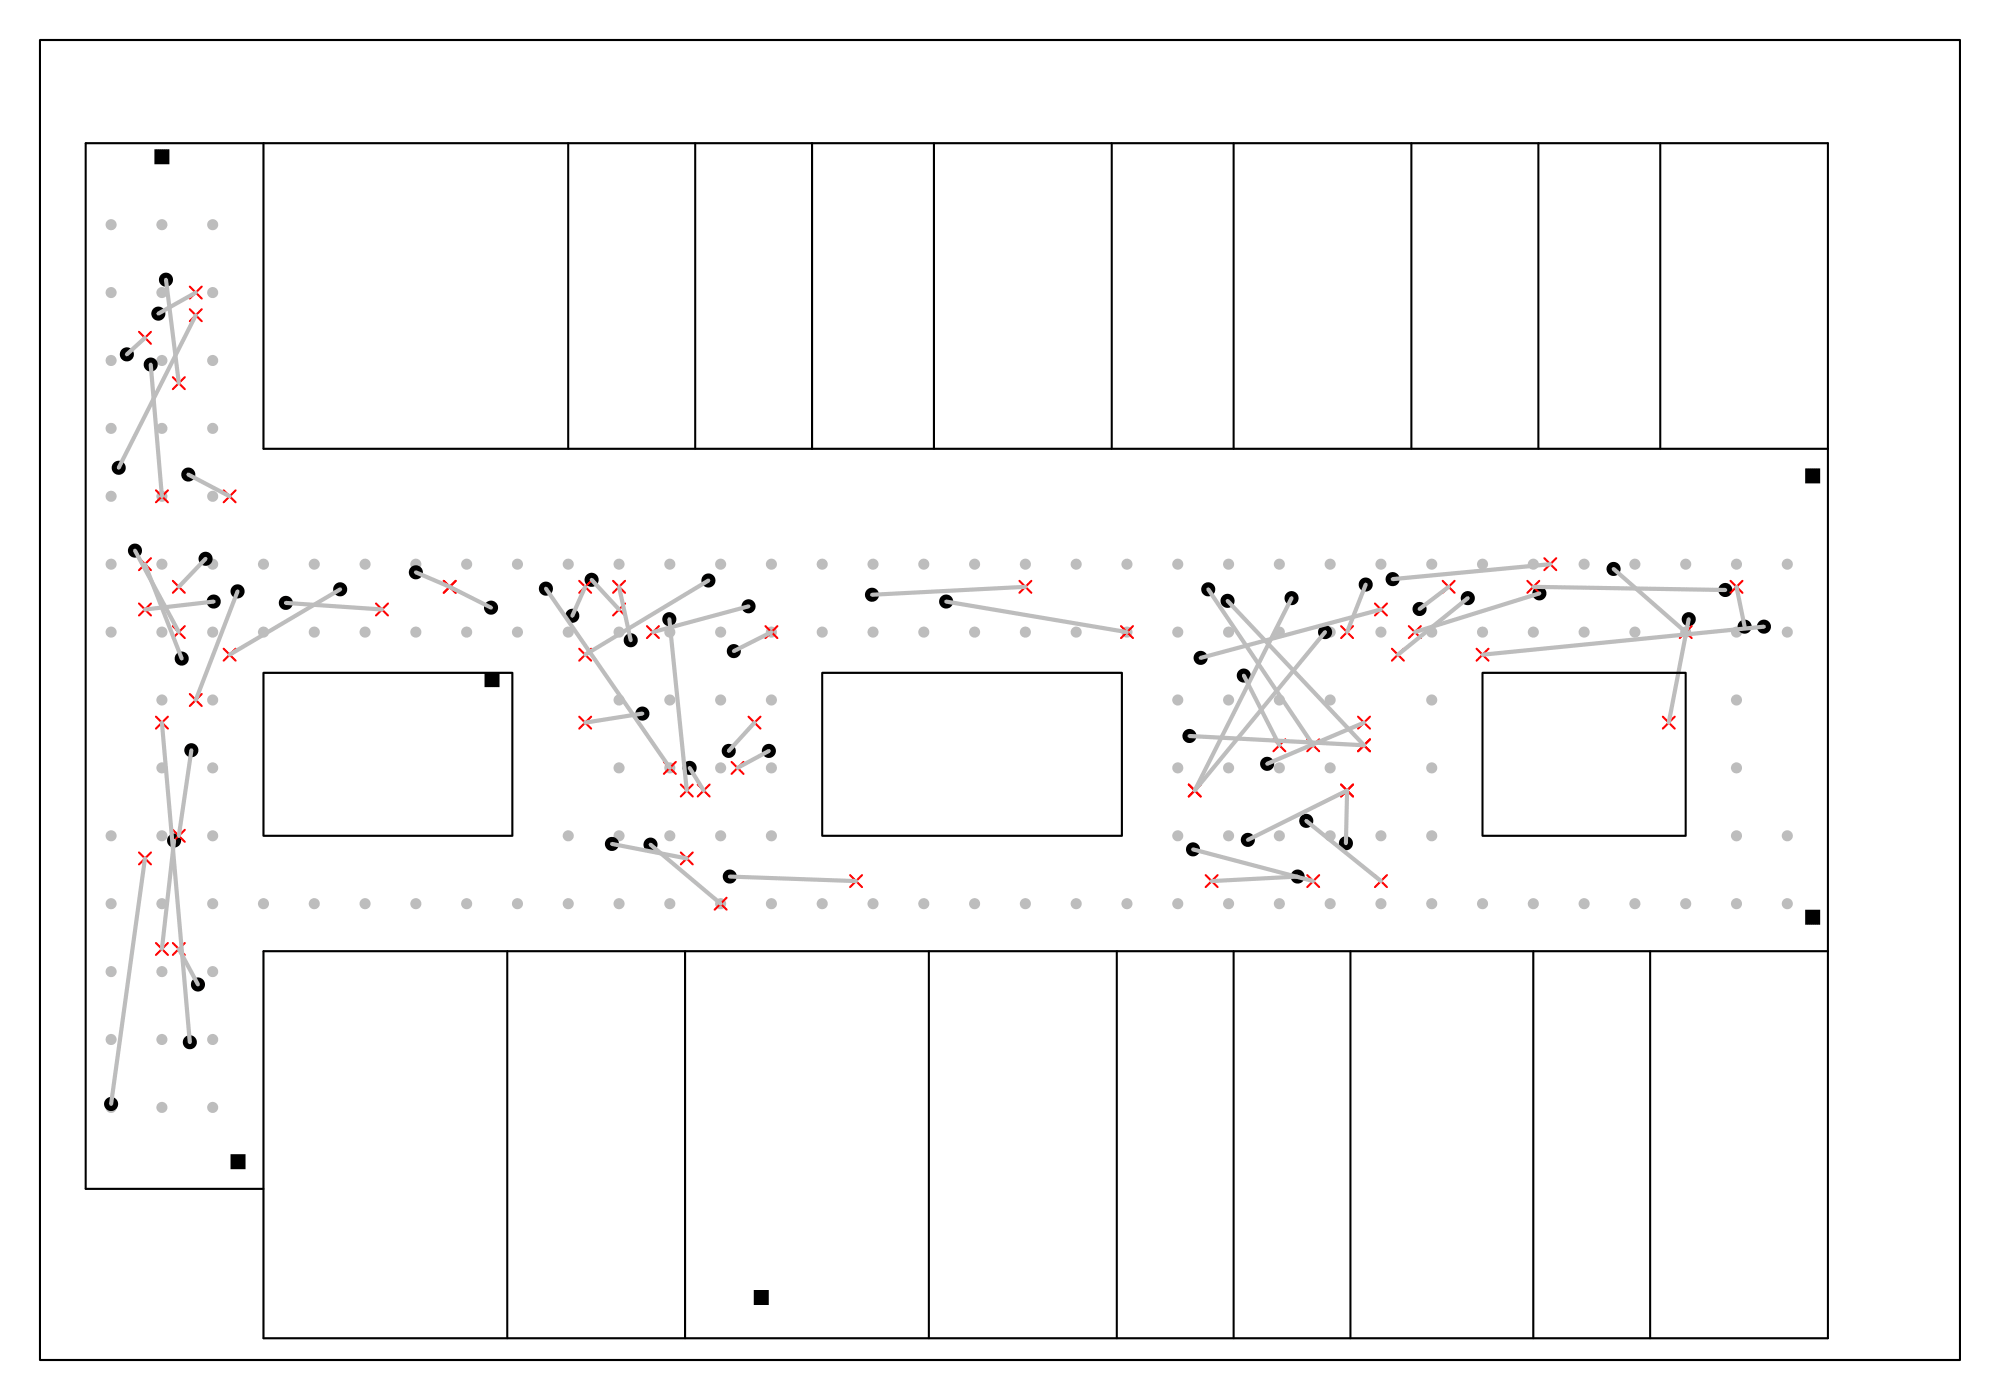
\includegraphics[width=\columnwidth]{img/Plot-K3FloorPlan-1.png}}
  \caption{Floor plan of estimated device locations when $k=3$}
  \label{fig: K3}
\end{figure}

\begin{figure}[htbp]
  \centerline{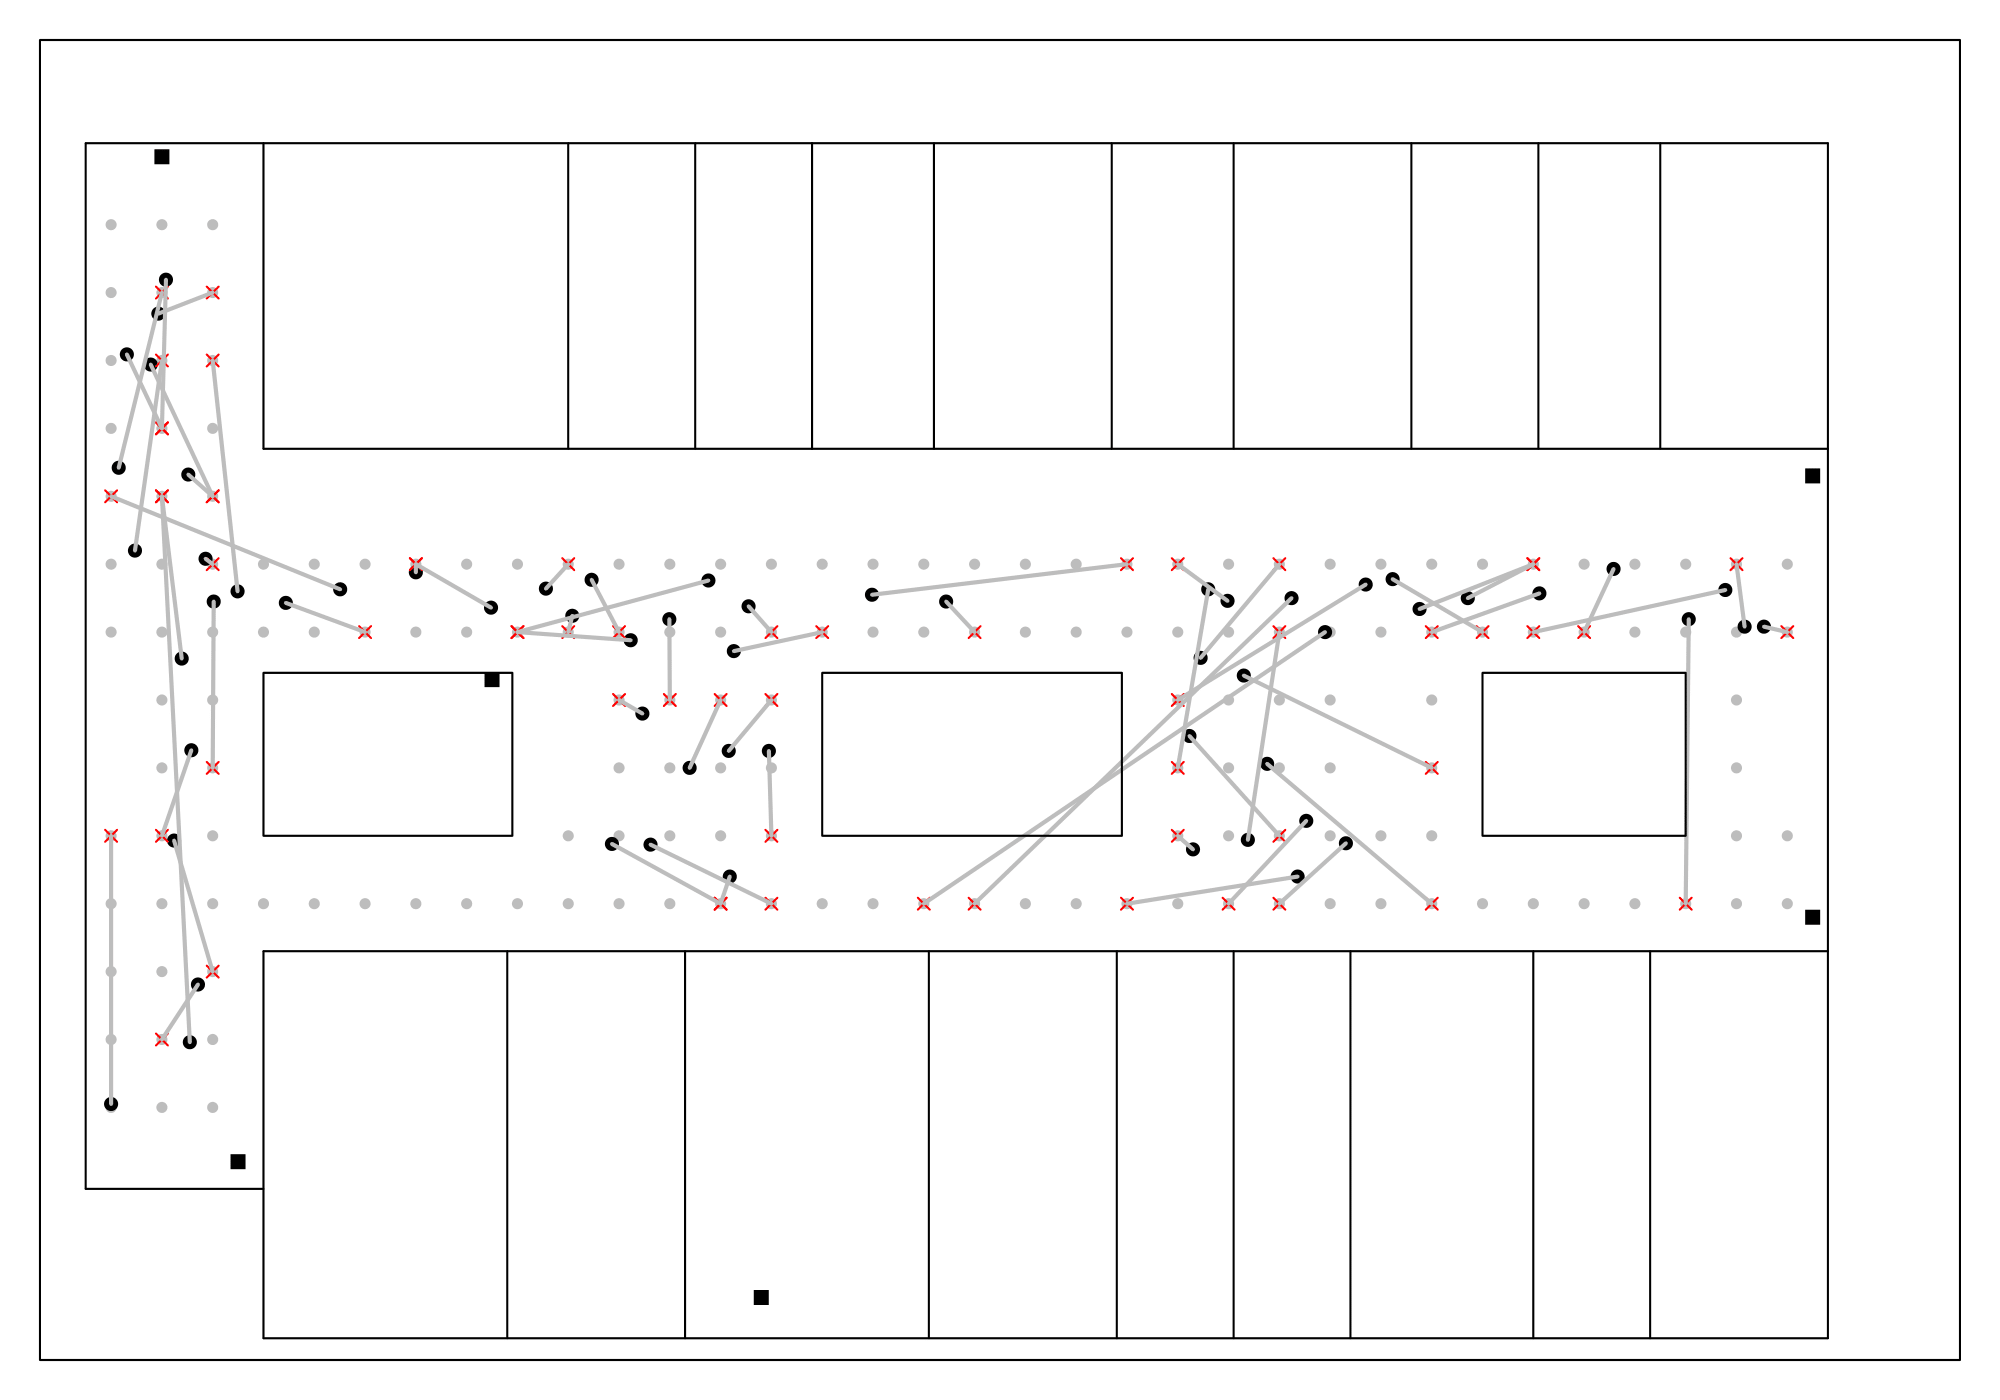
\includegraphics[width=\columnwidth]{img/Plot-K5FloorPlan-1.png}}
  \caption{Floor plan of estimated device locations when $k=5$}
  \label{fig: K5}
\end{figure}

The above 3 figures show the floor plan view of our dataset, the grids are the actual rooms, the gray points are the training dataset, the black points are the testing dataset, the black squares being the access points, and the black lines indicates the error between the actual and estimated positions.

We can see that $k=3$ shows a much smaller error in distance than $k=1$. While the plot for $k=5$ is similar to the plot for $k=1$, the average and median error in distance is actually smaller in $k=5$.

\begin{table}[htbp]
  \begin{tabular}{|l|c|c|}
  \hline
  # of $k$   & Average Error Distance & Median Error Distance \\ \hline
  $k=1$        & 2.517842 m             & 1.902775 m            \\ \hline
  $k=3$        & 1.931918 m             & 1.662997 m            \\ \hline
  $k=5$        & 1.769582 m             & 1.412887 m            \\ \hline
  \end{tabular}
\end{table}

%------------------------------------------------------------------------------------------------------------------------------------
% Evaluation
%------------------------------------------------------------------------------------------------------------------------------------
\section{Evaluation}
\begin{figure}[htbp]
  \centering
  \subfigure[Trilateration Prediction]{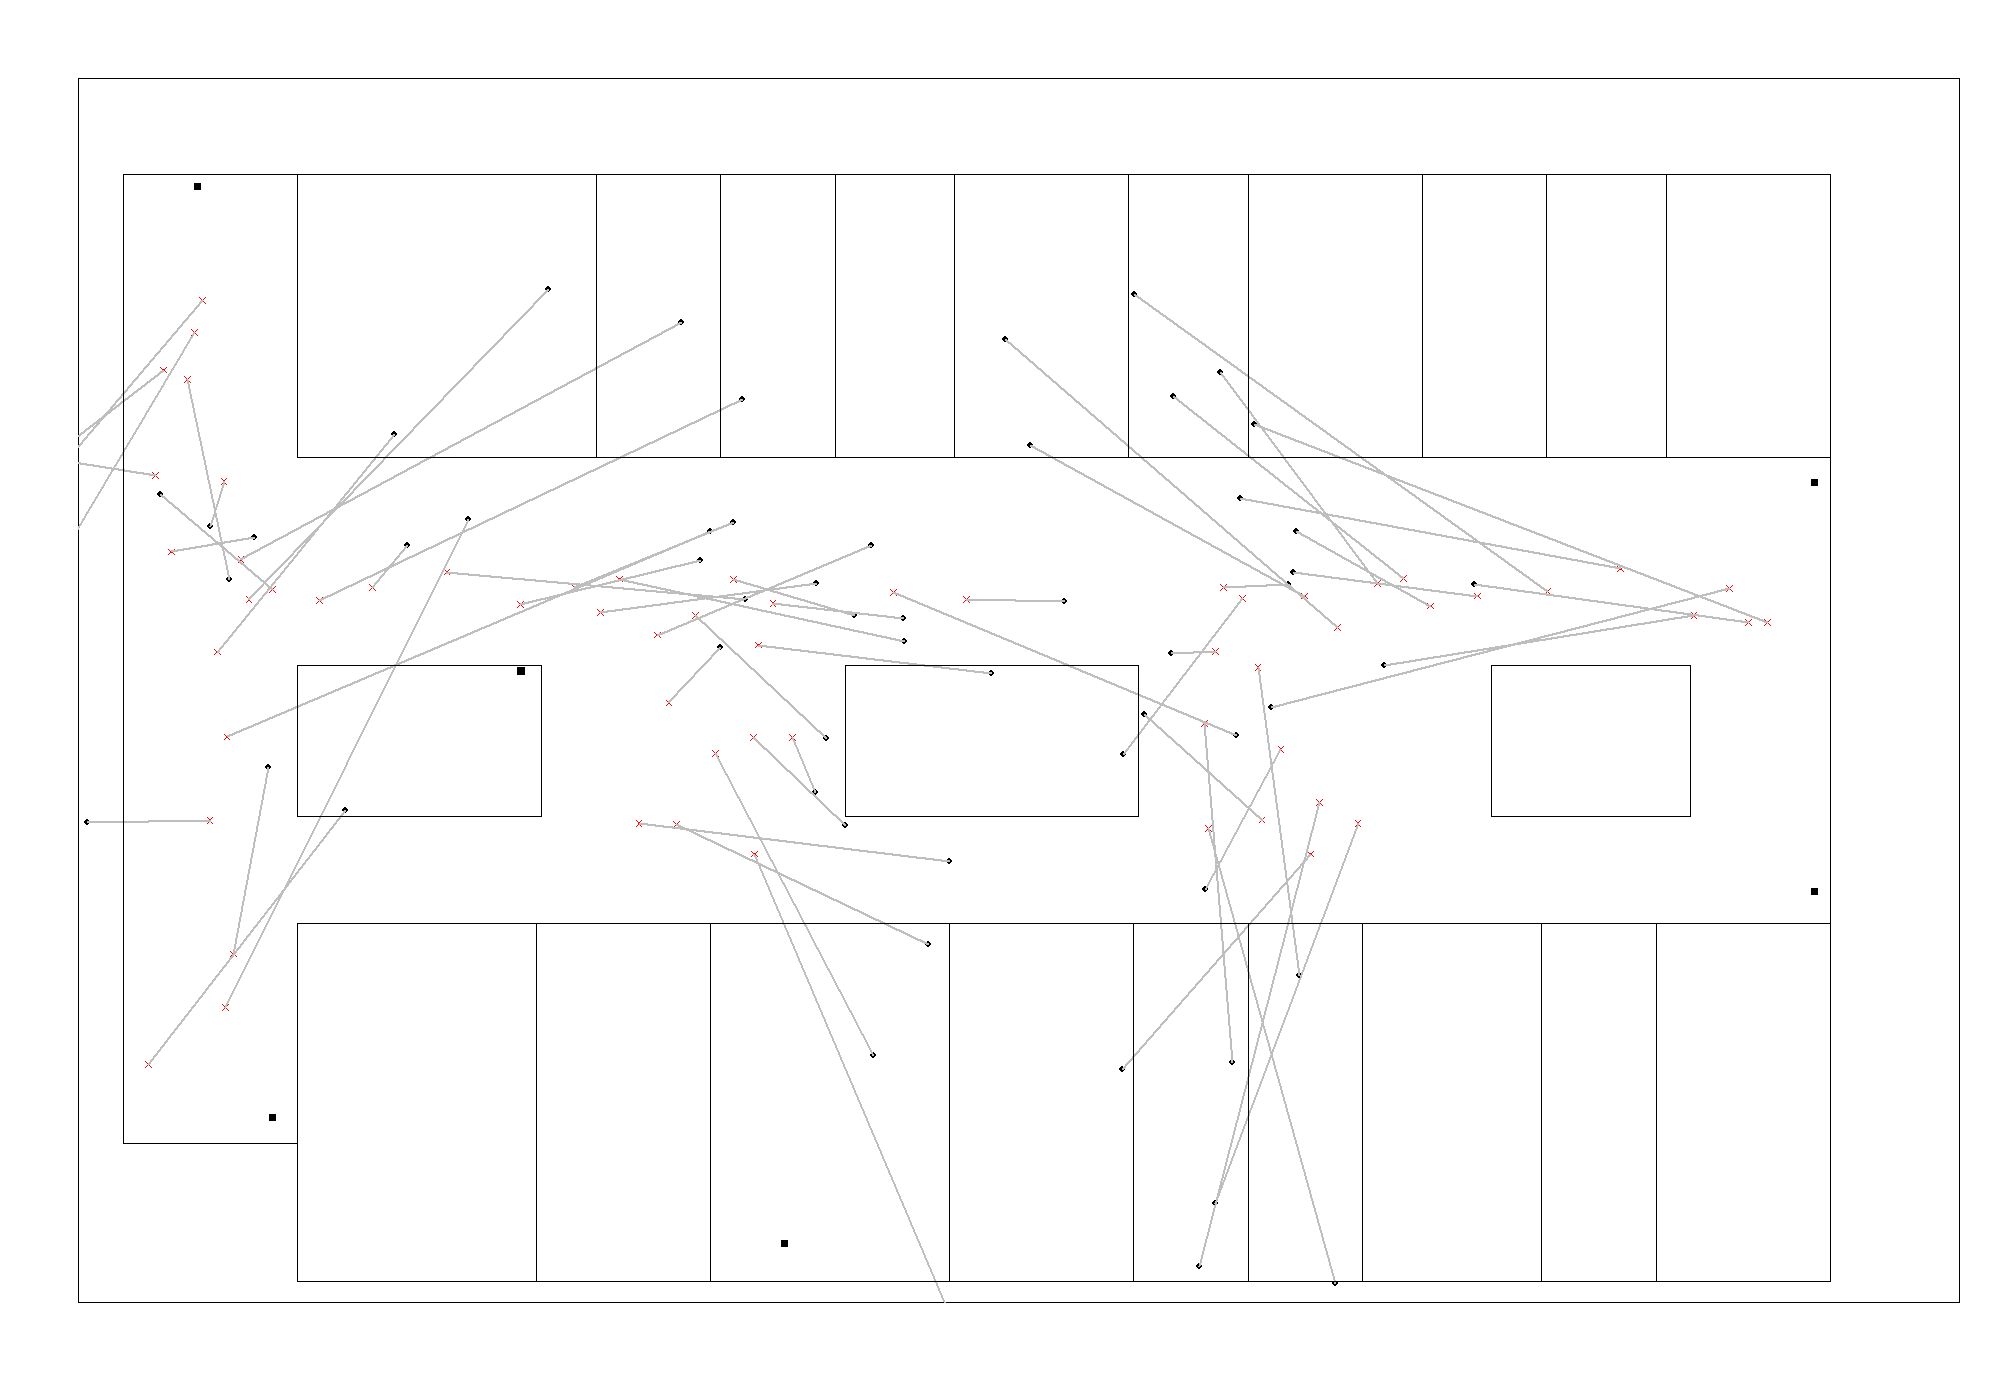
\includegraphics[width=0.24\textwidth]{img/Multilateration_Error.png}}
  \subfigure[KNN Prediction]{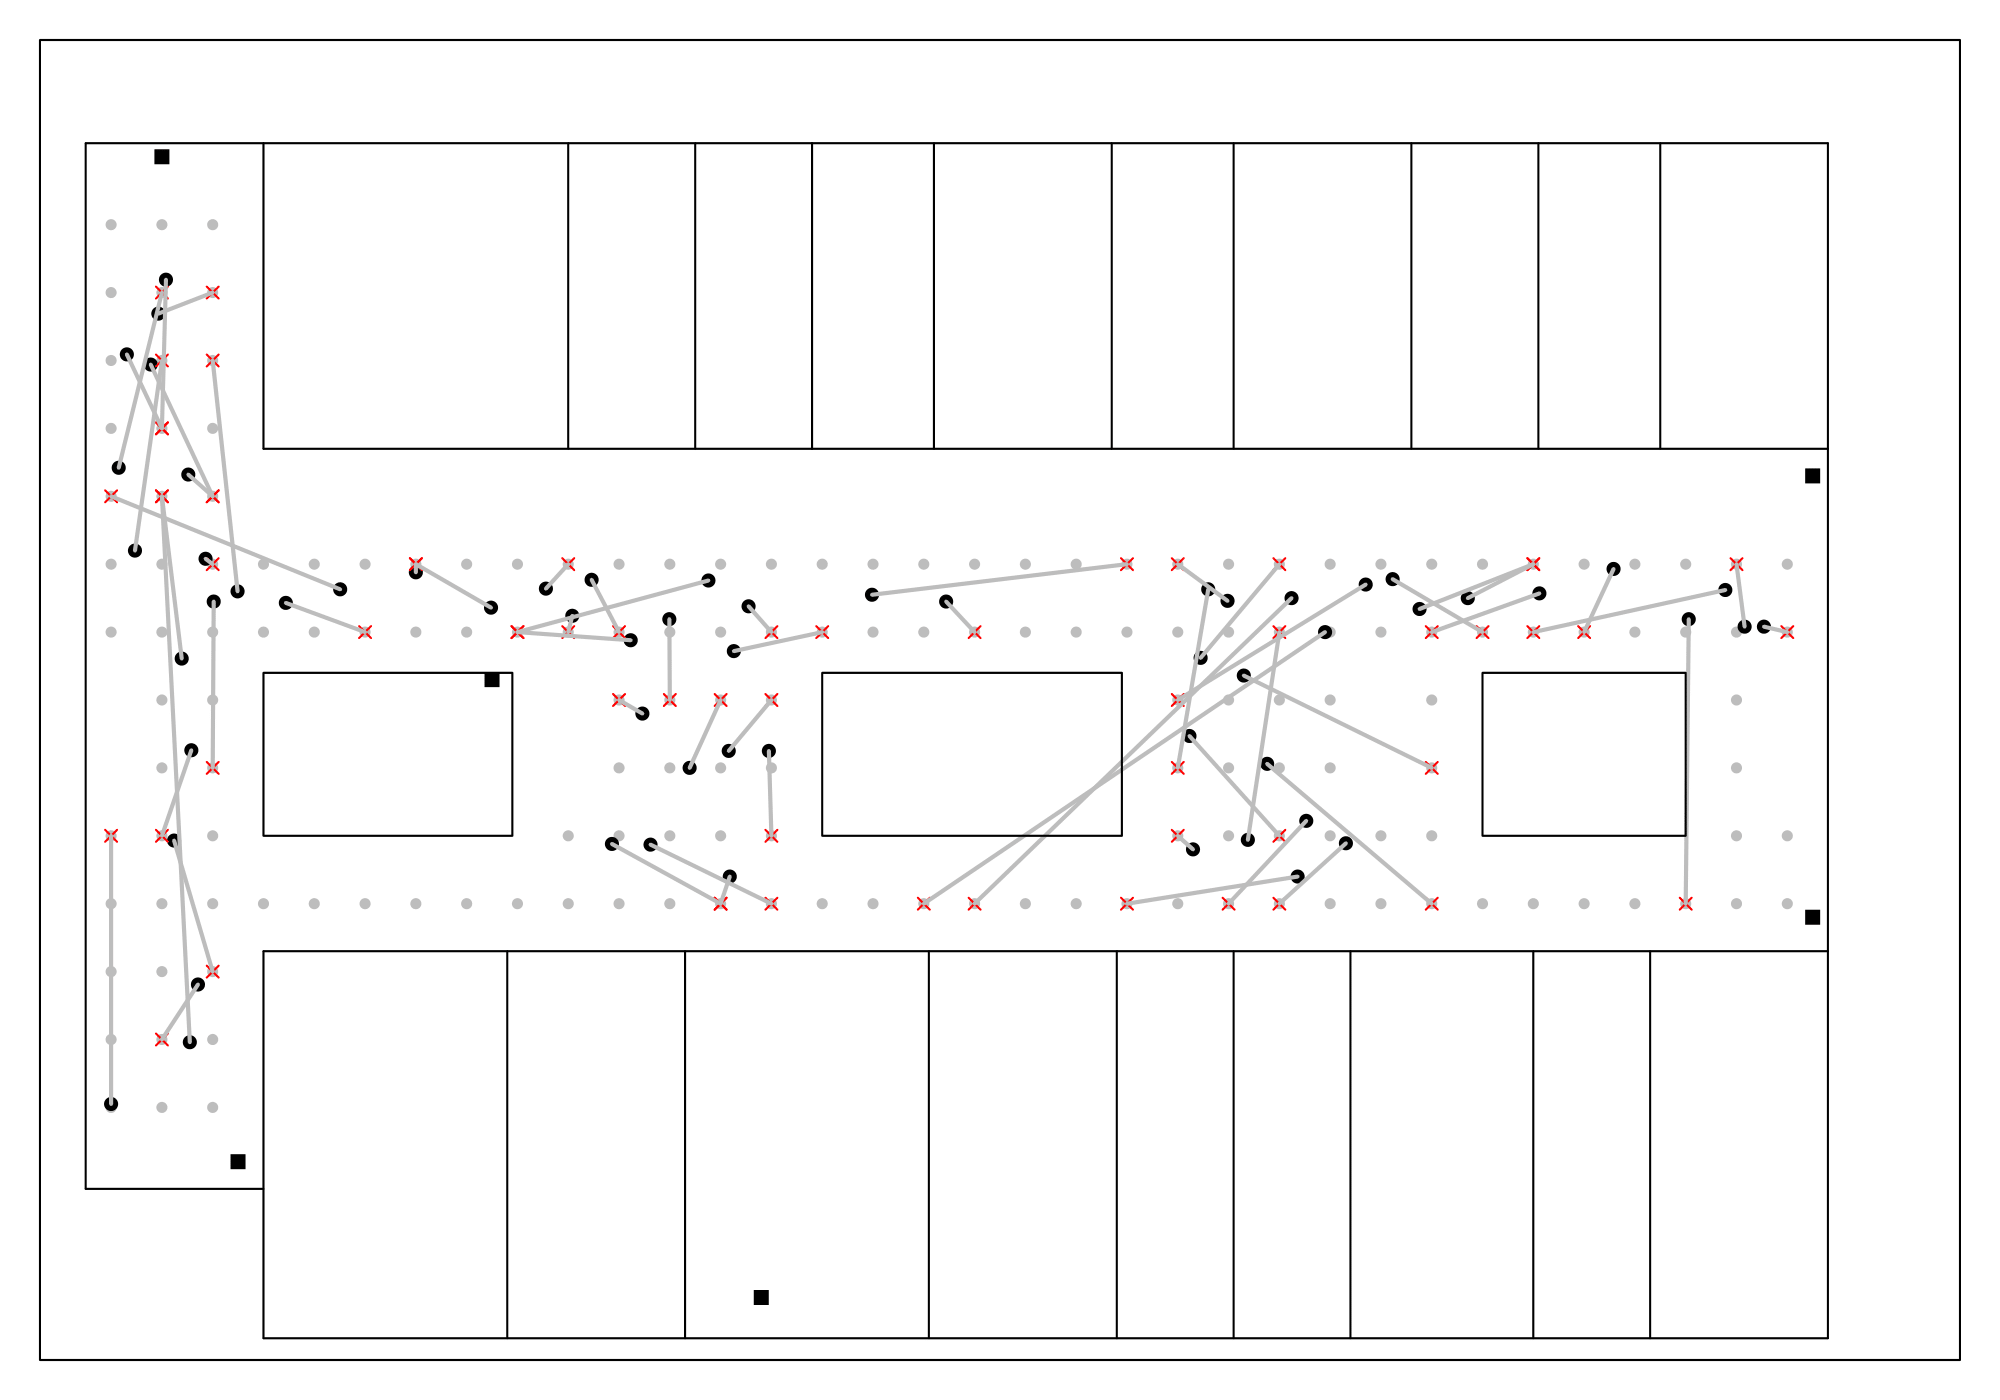
\includegraphics[width=0.24\textwidth]{img/Plot-K5FloorPlan-1.png}}
  \caption{Error of distance using 2 methods}
  \label{fig: Comparison}
\end{figure}

\begin{table}[htbp]
  \begin{tabular}{|l|c|c|}
  \hline
  Method        & Average Error Distance & Median Error Distance \\ \hline
  Trilateration & 4.832989 m             & 4.955922 m            \\ \hline
  KNN           & 2.517842 m             & 1.902775 m            \\ \hline
  \end{tabular}
\end{table}

%------------------------------------------------------------------------------------------------------------------------------------
% Conclusion
%------------------------------------------------------------------------------------------------------------------------------------
\section{Conclusion}
\begin{itemize}
  \item Extended version of the executive 
\end{itemize}



%------------------------------------------------------------------------------------------------------------------------------------
% Summary
%------------------------------------------------------------------------------------------------------------------------------------
\section{Summary}
\begin{itemize}
  \item Contextualization of results in light of project goals
  \item Make explicit connection to project background by following the implications of our results
\end{itemize}




%------------------------------------------------------------------------------------------------------------------------------------
% Reference
%------------------------------------------------------------------------------------------------------------------------------------
\begin{thebibliography}{00}
\bibitem{b1} 
\bibitem{b2} 
\bibitem{b3} 
\bibitem{b4} 
\bibitem{b5} 
\bibitem{b6} 
\bibitem{b7} 
\bibitem{b8} 
\bibitem{b9} 
\bibitem{b10} 
\end{thebibliography}
\vspace{12pt}



%------------------------------------------------------------------------------------------------------------------------------------
% Appendix
%------------------------------------------------------------------------------------------------------------------------------------
\section*{Appendix A: Data Tables}


\section*{Appendix B: Derivation of Equations}


\section*{Appendix C: Index}


\end{document}
